\section{Illustrative Examples}

We present examples in two groups. The first group consists of two analytically tractable cases where the inference problem is provably non-identifiable; these require no numerical computation and serve to illustrate the theoretical conditions of \Cref{section identifiability analysis}. The second group consists of two computational examples where all identifiability conditions are satisfied. For the numerical examples, we compare our Bayesian MCMC approach against the sparse-learning-CRN method of \cite{zhang2019learning}, which recovers propensity functions by solving an $\ell_1$-regularized least-squares problem (LASSO) over a polynomial basis using the FISTA algorithm. (All code and data are available at \href{https://github.com/ssindiUCM/BayesCRNInference}{BayesCRNInference}.)

%%--------------------------------------------------------------------
\subsection*{Structural Non-Identifiability: Two Illustrative Cases}
%%--------------------------------------------------------------------

The following two cases both satisfy \Cref{corollary structural non-identifiability by topological conditions} via a non-negative conservation law. In each case the violation of condition~\eqref{eq. sufficient and necessary conditions for structural identifiability} persists for all trajectory lengths: no amount of data can resolve the ambiguity. We do not report MCMC results for these cases; the non-identifiability is established analytically, and running the sampler would merely confirm that the posterior is diffuse over an equivalence class of parameter vectors.

\paragraph{First case: stoichiometric conservation law.} Following \cite{enciso2021identifiability}, consider two systems on species $(X_1,X_2)$ sharing the conservation law $X_1+X_2=2$:
\begin{equation}
X_1\xrightarrow{k_1=1}X_2,\quad X_2\xrightarrow{k_2=1}X_1
\label{eq:deg1}
\end{equation}
\begin{equation}
2X_1\xrightarrow{\lambda_1=2}X_1+X_2,\quad X_1+X_2\xrightarrow{\lambda_2=1}2X_1,\quad
X_1+X_2\xrightarrow{\lambda_3=1}2X_2,\quad 2X_2\xrightarrow{\lambda_4=2}X_1+X_2
\label{eq:deg2}
\end{equation}
The conservation law confines the state space to $\{(2,0),(1,1),(0,2)\}$. Table~\ref{tab:degenerate} shows that both systems produce identical propensities at every accessible state, so condition~\eqref{eq. sufficient and necessary conditions for structural identifiability} is violated for every member of the interpolating family $\theta(\alpha)=\alpha\,\theta_{\text{Sys.1}}+(1-\alpha)\,\theta_{\text{Sys.2}}$. The conservation vector $c=(1,1)^\top$ exists and the channel $\xi_\ell=(-1,+1)$ contains the unimolecular reaction $X_1\to X_2$ ($\|\nu\|_1=1$), satisfying condition~(2) of \Cref{corollary structural non-identifiability by topological conditions}. Structural non-identifiability follows regardless of trajectory length.

\begin{table}[h!]
\centering
\begin{tabular}{|c|c|c|c|}
\hline
State $(X_1,X_2)$ & $(\Delta X_1,\Delta X_2)$ & Sys.~\eqref{eq:deg1} propensity & Sys.~\eqref{eq:deg2} propensity \\
\hline
$(2,0)$ & $(-1,+1)$ & $k_1\cdot 2=2$ & $\lambda_1\cdot\tfrac{2(2-1)}{2}=2$ \\
$(1,1)$ & $(-1,+1)$ & $k_1\cdot 1=1$ & $\lambda_3\cdot 1\cdot 1=1$ \\
$(1,1)$ & $(+1,-1)$ & $k_2\cdot 1=1$ & $\lambda_2\cdot 1\cdot 1=1$ \\
$(0,2)$ & $(+1,-1)$ & $k_2\cdot 2=2$ & $\lambda_4\cdot\tfrac{2(2-1)}{2}=2$ \\
\hline
\end{tabular}
\caption{Propensities for Systems~\eqref{eq:deg1} and~\eqref{eq:deg2} with $X_1+X_2=2$. The two systems are indistinguishable at every accessible state.}
\label{tab:degenerate}
\end{table}

\paragraph{Second case: catalyst species.} Consider the two-species system
\begin{equation}
\emptyset\xrightarrow{k_1=1}X_1,\quad X_1\xrightarrow{k_2=1}2X_1,\quad X_1+X_2\xrightarrow{k_3=0.1}X_2,
\label{eq:example2}
\end{equation}
with propensities $a_1=k_1$, $a_2=k_2 X_1(X_1{-}1)/2$, $a_3=k_3 X_1 X_2$. Since no reaction in~\eqref{eq:example2} produces or degrades $X_2$, the species acts as a permanent catalyst: $X_2(t)=c_2$ for all $t$. This constitutes a conservation law with $c=(0,1)^\top$, and \Cref{corollary structural non-identifiability by topological conditions} applies again. In the channel $\xi_\ell=(-1,0)$, the candidate reaction $X_1\to\emptyset$ is unimolecular ($\|\nu\|_1=1$), satisfying condition~(2). The propensities $k\,X_1$ (for $X_1\to\emptyset$) and $k'\,c_2 X_1$ (for $X_1+X_2\to X_2$) are proportional for all visited states, so the full-rank condition~\eqref{eq. local cancavity check} fails and any pair $(\tilde k_1,\tilde k_3)$ with $\tilde k_1+\tilde k_3 c_2=k_3 c_2$ is equally consistent with the data. In contrast to the first case, where non-identifiability arises from the topology of the state space, here it arises from collinearity of the propensity functions - but both are structural, persisting in every trajectory generated by these networks.

\subsubsection*{Numerical Example 1: Predator-Prey System}

Both numerical examples satisfy all identifiability conditions of \Cref{section identifiability analysis}. Throughout, Bayesian MCMC is run with a spike-and-slab prior ($\pi=0.75$, $\alpha=2$, $\beta=0.25$), 500{,}000 iterations, 50{,}000 burn-in, thinning by 100, and rates initialized from $U[0.001,2.0]$, with covariance updated adaptively every 10 iterates. For comparison, the LASSO method of \cite{zhang2019learning} is applied at regularization strength $\lambda=0.01$ unless stated otherwise.

We consider the stochastic Lotka-Volterra system with prey $A$ and predator $B$:
\begin{equation}
A\xrightarrow{k_1=1.0}2A,\quad
A\xrightarrow{k_2=0.1}\emptyset,\quad
A+B\xrightarrow{k_3=0.01}2B,\quad
B\xrightarrow{k_4=0.5}\emptyset,
\label{eq:predprey}
\end{equation}
with mass-action propensities $\lambda_1=k_1 A$, $\lambda_2=k_2 A$, $\lambda_3=k_3 AB$, $\lambda_4=k_4 B$. The deterministic equilibrium is $(A^*,B^*)=(50,90)$. Starting from $(A,B)=(100,50)$, the system is simulated over $T=40$, yielding 5{,}805 events across four stoichiometric channels. The large initial displacement from equilibrium drives pronounced oscillatory dynamics, with stochastic prey extinction occurring near $t=39.8$.

We search over all unimolecular and bimolecular candidate reactions for the two species system under the assumption of mass action kinetics. The rank condition~\eqref{eq. local cancavity check} is satisfied for each active channel. Figure~\ref{fig:predprey_traj} shows the simulated trajectory. Table~\ref{tab:predprey_detail} shows all candidate reactions considered for each stoichiometric channel, together with the posterior results. Our Bayesian approach correctly identifies all four stoichiometric channels, with posterior means within 2\% of the true rates and $\Pr(\text{off})=0$ for all active reactions. All inactive candidate reactions receive $\Pr(\text{off})\approx 1$.

\begin{figure}[htbp]
\centering
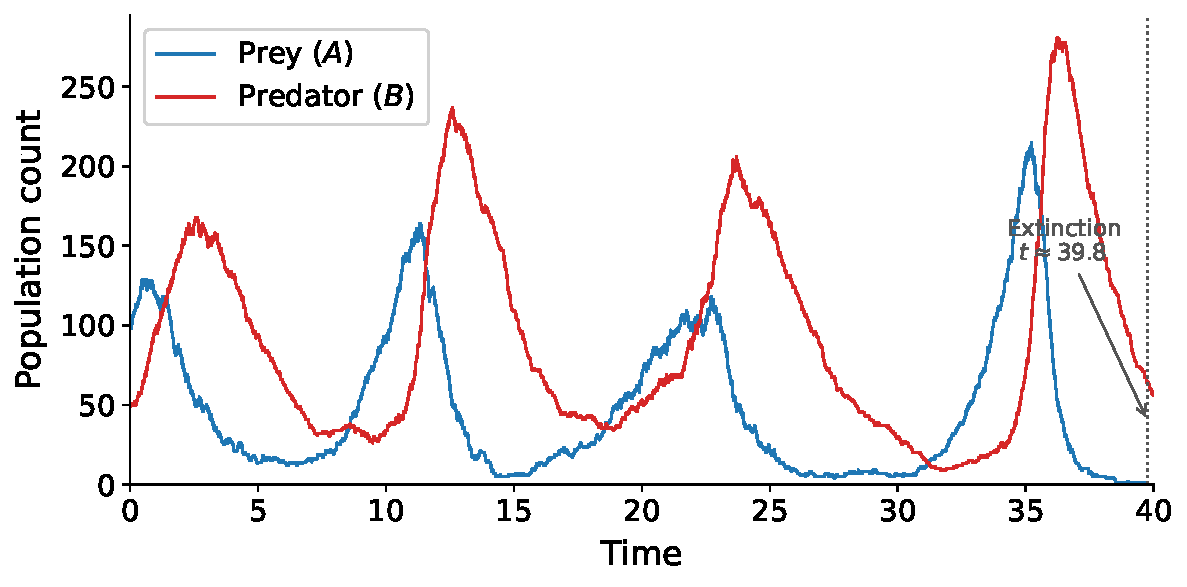
\includegraphics[width=0.85\textwidth]{fig_predprey_traj}
\caption{Stochastic trajectory of the predator-prey system~\eqref{eq:predprey} simulated over $T=40$ from initial state $(A,B)=(100,50)$. Prey ($A$, blue) and predator ($B$, red) undergo pronounced oscillations driven by the large displacement from the deterministic equilibrium $(A^*,B^*)=(50,90)$. Prey extinction occurs near $t\approx 39.8$ (dotted line), yielding 5{,}805 observed events across four stoichiometric channels.}
\label{fig:predprey_traj}
\end{figure}

% Table 4 — Predator-prey Bayesian detail
\begin{table}[htbp]
\centering
\small
\caption{Predator-prey inference at $T=40$ (5{,}805 events total). All candidate mass-action reactions for each stoichiometric channel $\xi_\ell$ are shown. $k^*$: true rate (bold if active). $\hat{k}$: posterior mean (95\% credible interval). $\Pr(\text{off})$: spike-and-slab exclusion probability. LASSO propensity at $\lambda=0.01$. Entries marked ``---'' have $\Pr(\text{off})>0.99$: the posterior is overwhelmingly concentrated on the spike component (rate $=0$), so the credible interval collapses to a point at zero and is not reported. $^\dagger$~Mechanistically impossible under mass-action kinetics.}
\label{tab:predprey_detail}
\begin{tabular}{l l r r l r l}
\toprule
$\xi_\ell$ & Candidate reaction & $k^*$ & Events & $\hat{k}$\;(95\% CI) & $\Pr(\text{off})$ & LASSO \\
\midrule
\multirow{3}{*}{$(+1,\;0)$} & $\emptyset\to A$ & $0$ & 1933 & --- & $0.995$ &  \\
 & $A\to 2A$ & \textbf{1.0000} &  & $1.0024\;(0.9587,\,1.0480)$ & $0.000$ & $0.969\,A$ \\
 & $B\to A+B$ & $0$ &  & --- & $1.000$ &  \\
\midrule
\multirow{3}{*}{$(-1,\;0)$} & $A\to \emptyset$ & \textbf{0.1000} & 190 & $0.0995\;(0.0859,\,0.1140)$ & $0.000$ & $0.018\,A + 0.036\,B^{\,\dagger}$ \\
 & $2A\to A$ & $0$ &  & --- & $1.000$ &  \\
 & $A+B\to B$ & $0$ &  & --- & $1.000$ &  \\
\midrule
\multirow{3}{*}{$(-1,+1)$} & $A\to B$ & $0$ & 1843 & --- & $1.000$ &  \\
 & $2A\to A+B$ & $0$ &  & --- & $1.000$ &  \\
 & $A+B\to 2B$ & \textbf{0.0100} &  & $0.0101\;(0.0096,\,0.0105)$ & $0.000$ & $0.010\,AB$ \\
\midrule
\multirow{3}{*}{$(0,\;-1)$} & $B\to \emptyset$ & \textbf{0.5000} & 1837 & $0.4918\;(0.4705,\,0.5144)$ & $0.000$ & $0.497\,B$ \\
 & $2B\to B$ & $0$ &  & --- & $1.000$ &  \\
 & $A+B\to A$ & $0$ &  & --- & $1.000$ &  \\
\bottomrule
\end{tabular}
\end{table}

The LASSO was applied with a polynomial basis of degree at most 2, $\{1,A,B,A^2,AB,B^2\}$ at regularization strength $\lambda = 0.01$. This method performs well on the channels $(+1,0)$, $(-1,+1)$, and $(0,-1)$, but fails on channel $(-1,0)$ corresponding to $A\to\emptyset$. Rather than recovering a propensity proportional to $A$, it returns $0.018\,A+0.036\,B$, assigning the larger coefficient to $B$. We note that this would be mechanistically impossible under the assumption of mass-action kinetics. However, this failure has an understandable structural cause. Near the deterministic equilibrium $B^*=90>A^*=50$, values of $B$ are systematically larger than values of $A$, so assigning weight to $B$ achieves a similar propensity contribution at lower $\ell_1$ cost. The oscillation-induced correlation between $A$ and $B$ further compounds this, and the low event count (190 jumps) provides insufficient signal to overcome it. Because the Bayesian approach works directly in the space of reaction rates under mass-action constraints (rather than fitting unconstrained polynomial coefficients) it is not susceptible to this scale imbalance. 

We note that \cite{zhang2019learning} also demonstrated their method on a two-species predator-prey system with the same four reaction types, using 100 independent trajectories of length $T=10$ and a smaller regularization parameter $\lambda = 0.0001$; the substantially larger data volume (equivalent to 1{,}000 total time units versus our single trajectory of length $T=40$) and the absence of extinction events likely reduce the oscillation-induced correlation between $A$ and $B$ that causes the failure on channel $(-1,0)$. Our comparison thus reflects a regime where data are limited and the trajectory is far from stationarity, which is precisely where the structural constraints of the Bayesian formulation provide the greatest advantage.

\subsubsection*{Numerical Example 2: Randomly Generated Reaction Network}

Using the same MCMC and LASSO settings as in the previous example (polynomial order 2), we assess performance at scale with a four-species system $(A,B,X,Y)$, enumerating all unimolecular and bimolecular reactions to form a candidate space of 130 stoichiometric channels. Twenty reactions are selected at random (with 4 channels chosen to contain 2 active reactions each), and rate parameters are independently drawn from $\mathrm{Gamma}(2.6,\,0.4)$. A single trajectory is simulated from $(A,B,X,Y)=(5,5,5,5)$ over $T\in\{100,200,400\}$; all species remain at low copy numbers throughout (maximum count 20), as shown in Figure~\ref{fig:example5_traj}, making structural identification from short trajectories particularly challenging.

Results in Tables~\ref{tab:bayes-detail-T100}--\ref{tab:lasso-lambda-sweep} show that the spike-and-slab prior achieves exact structural recovery at all three time horizons: every inactive reaction receives $\Pr(\text{off})=1.000$ and every active reaction $\Pr(\text{off})=0.000$, with posterior widths narrowing as $T$ increases. This includes the four channels containing two simultaneously active reactions, where both reactions are correctly identified in each case. Even the $-2A$ channel, observed only 60 times at $T=100$, is correctly identified with $\Pr(\text{off})=0$ and a posterior mean within 3\% of the true rate (Table~\ref{tab:bayes-detail-T100}).

At $T=100$, the Bayesian method achieves lower $L^2$ propensity error than LASSO on every channel (errors $0.008$--$0.168$ vs.\ $0.143$--$0.991$; Table~\ref{tab:comparison-l2}). Notably, LASSO errors improve little or worsen from $T=200$ to $T=400$ on several channels (e.g., $-2A,\!+1X,\!+1Y$: $0.754\to0.851\to0.993$), whereas Bayesian errors consistently shrink with more data. A sweep over $\lambda\in\{0.001,0.005,0.01,0.05,0.1,0.5\}$ confirms that no single regularization strength minimizes error across all channels simultaneously: weak-reaction channels require small $\lambda$ to avoid over-shrinkage, while noisy channels require large $\lambda$ for suppression (Table~\ref{tab:lasso-lambda-sweep}). The Bayesian framework resolves this automatically through the spike-and-slab prior, adapting to each channel's evidence without global tuning.


\begin{figure}[htbp]
\centering
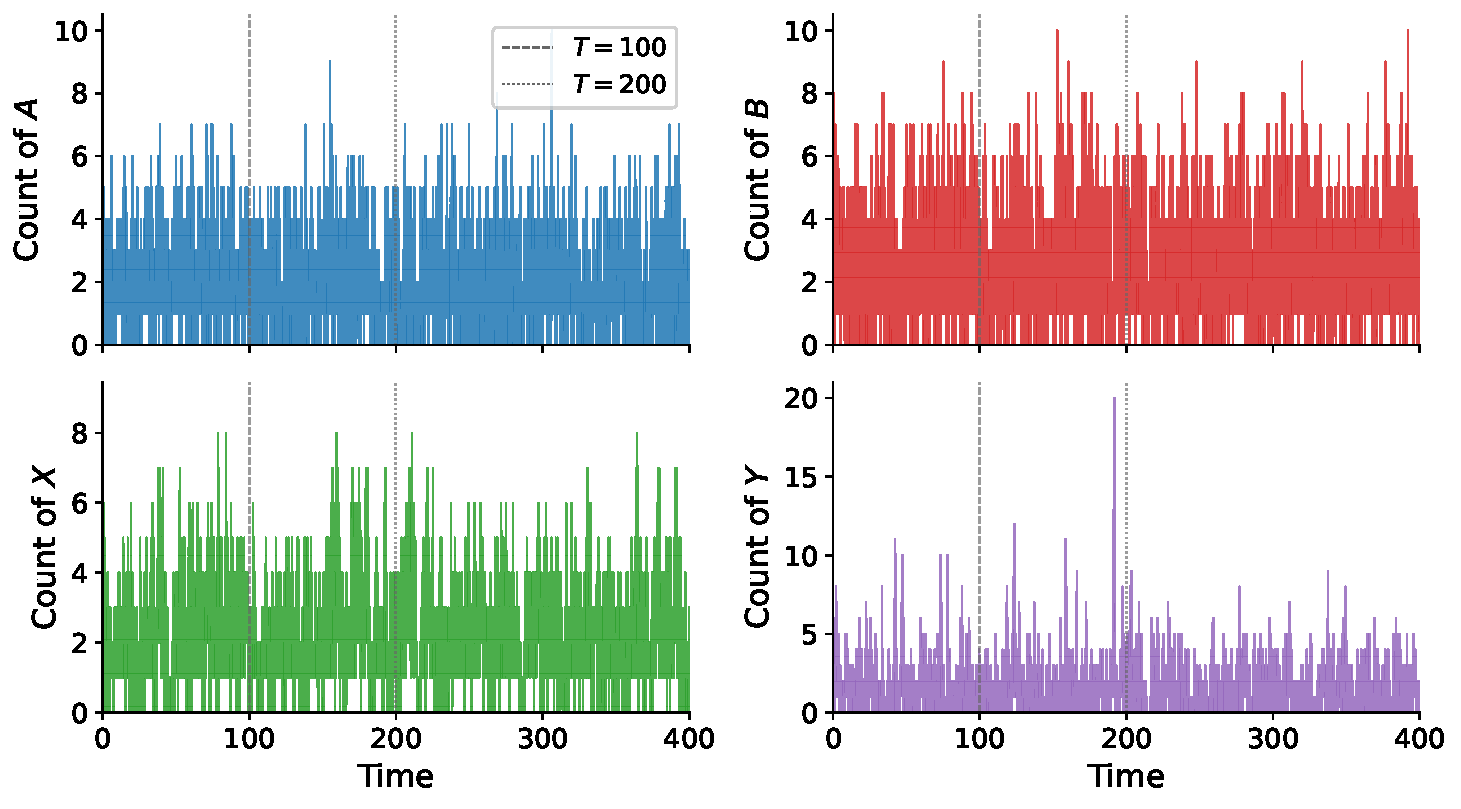
\includegraphics[width=\textwidth]{fig_example5_traj}
\caption{Stochastic trajectory of the randomly generated four-species system $(A,B,X,Y)$, simulated from $(5,5,5,5)$ over $T=400$. Each panel shows one species; the dashed and dotted vertical lines mark the $T=100$ and $T=200$ observation horizons used in the inference experiments. All species remain at low copy numbers throughout, making structural identification from short trajectories challenging.}
\label{fig:example5_traj}
\end{figure}

% Bayesian detail at T=100, T=200, T=400
% Bayesian spike-and-slab detail T=100
\begin{table}[htbp]
\centering
\small
\caption{Bayesian spike-and-slab posterior estimates, $T=100$. Stoichiometric change $\xi_\ell$ and observed event count (Obs) are shown once per channel. True rate $k^*$ is bold for active reactions. $\hat{k}$ and 95\% credible interval are combined. Candidates with $\Pr(\text{off})>0.99$ are omitted.}
\label{tab:bayes-detail-T100}
\begin{tabular}{lrlrll}
\toprule
\textbf{Change} & \textbf{Obs} & \textbf{Reaction} & \textbf{True $k^*$} & $\hat{k}$\;(95\% CI) & $\Pr(\text{off})$ \\
\midrule
$-2A$ & 60 & $2A \to \emptyset$ & \textbf{0.4528} & 0.4416\;[0.341,\,0.559] & 0.0000 \\
\midrule
$-2A$, $+1X$, $+1Y$ & 129 & $2A \to X+Y$ & \textbf{1.0206} & 0.9363\;[0.783,\,1.105] & 0.0000 \\
\midrule
$-2A$, $+1B$ & 230 & $2A \to B$ & \textbf{1.5713} & 1.6576\;[1.451,\,1.869] & 0.0000 \\
\midrule
$-2B$, $+1X$ & 615 & $2B \to X$ & \textbf{1.9789} & 2.0576\;[1.904,\,2.221] & 0.0000 \\
\midrule
$-1X$, $+1Y$ & 138 & $X+Y \to 2Y$ & \textbf{0.4887} & 0.5338\;[0.446,\,0.625] & 0.0000 \\
\midrule
\multirow{2}{*}{$-1Y$} & \multirow{2}{*}{310} & $A+Y \to A$ & \textbf{0.5897} & 0.4821\;[0.344,\,0.635] & 0.0000 \\
 &  & $X+Y \to X$ & \textbf{0.7676} & 0.7801\;[0.638,\,0.925] & 0.0000 \\
\midrule
\multirow{2}{*}{$+1Y$} & \multirow{2}{*}{184} & $A \to A+Y$ & \textbf{0.2803} & 0.2617\;[0.164,\,0.373] & 0.0002 \\
 &  & $Y \to 2Y$ & \textbf{1.0673} & 0.9431\;[0.772,\,1.125] & 0.0000 \\
\midrule
$+1X$, $-1Y$ & 136 & $A+Y \to A+X$ & \textbf{0.6456} & 0.6117\;[0.514,\,0.716] & 0.0000 \\
\midrule
\multirow{2}{*}{$+1B$, $-1X$} & \multirow{2}{*}{427} & $2X \to B+X$ & \textbf{1.2593} & 1.2039\;[1.003,\,1.413] & 0.0000 \\
 &  & $A+X \to A+B$ & \textbf{0.4167} & 0.3291\;[0.226,\,0.443] & 0.0000 \\
\midrule
$+1B$, $-1X$, $+1Y$ & 317 & $X \to B+Y$ & \textbf{1.2783} & 1.3700\;[1.227,\,1.526] & 0.0000 \\
\midrule
\multirow{2}{*}{$+1B$, $-1Y$} & \multirow{2}{*}{326} & $A+Y \to A+B$ & \textbf{0.4221} & 0.3658\;[0.234,\,0.512] & 0.0000 \\
 &  & $X+Y \to B+X$ & \textbf{0.9061} & 0.9419\;[0.793,\,1.095] & 0.0000 \\
\midrule
\multirow{2}{*}{$+1B$} & \multirow{2}{*}{378} & $A \to A+B$ & \textbf{1.0464} & 1.2137\;[0.948,\,1.488] & 0.0000 \\
 &  & $X \to B+X$ & \textbf{0.7167} & 0.7369\;[0.553,\,0.937] & 0.0000 \\
\midrule
$+2B$ & 64 & $\emptyset \to 2B$ & \textbf{0.6782} & 0.6586\;[0.511,\,0.824] & 0.0000 \\
\midrule
$+1A$, $-1B$ & 580 & $B \to A$ & \textbf{2.2031} & 2.2523\;[2.072,\,2.445] & 0.0007 \\
\midrule
$+1A$ & 255 & $A \to 2A$ & \textbf{1.5168} & 1.4763\;[1.302,\,1.661] & 0.0000 \\
\bottomrule
\end{tabular}
\end{table}
% Bayesian spike-and-slab detail T=200
\begin{table}[htbp]
\centering
\small
\caption{Bayesian spike-and-slab posterior estimates, $T=200$. Stoichiometric change $\xi_\ell$ and observed event count (Obs) are shown once per channel. True rate $k^*$ is bold for active reactions. $\hat{k}$ and 95\% credible interval are combined. Candidates with $\Pr(\text{off})>0.99$ are omitted.}
\label{tab:bayes-detail-T200}
\begin{tabular}{lrlrll}
\toprule
\textbf{Change} & \textbf{Obs} & \textbf{Reaction} & \textbf{True $k^*$} & $\hat{k}$\;(95\% CI) & $\Pr(\text{off})$ \\
\midrule
$-2A$ & 115 & $2A \to \emptyset$ & \textbf{0.4528} & 0.4230\;[0.351,\,0.503] & 0.0000 \\
\midrule
$-2A$, $+1X$, $+1Y$ & 263 & $2A \to X+Y$ & \textbf{1.0206} & 0.9590\;[0.849,\,1.078] & 0.0000 \\
\midrule
$-2A$, $+1B$ & 452 & $2A \to B$ & \textbf{1.5713} & 1.6443\;[1.499,\,1.797] & 0.0000 \\
\midrule
$-2B$, $+1X$ & 1185 & $2B \to X$ & \textbf{1.9789} & 2.0292\;[1.914,\,2.147] & 0.0000 \\
\midrule
$-1X$, $+1Y$ & 252 & $X+Y \to 2Y$ & \textbf{0.4887} & 0.5010\;[0.444,\,0.562] & 0.0000 \\
\midrule
\multirow{2}{*}{$-1Y$} & \multirow{2}{*}{626} & $A+Y \to A$ & \textbf{0.5897} & 0.5647\;[0.455,\,0.685] & 0.0000 \\
 &  & $X+Y \to X$ & \textbf{0.7676} & 0.7817\;[0.677,\,0.891] & 0.0000 \\
\midrule
\multirow{2}{*}{$+1Y$} & \multirow{2}{*}{398} & $A \to A+Y$ & \textbf{0.2803} & 0.2773\;[0.204,\,0.358] & 0.0000 \\
 &  & $Y \to 2Y$ & \textbf{1.0673} & 1.0147\;[0.890,\,1.146] & 0.0000 \\
\midrule
$+1X$, $-1Y$ & 264 & $A+Y \to A+X$ & \textbf{0.6456} & 0.6411\;[0.567,\,0.718] & 0.0000 \\
\midrule
\multirow{2}{*}{$+1B$, $-1X$} & \multirow{2}{*}{860} & $2X \to B+X$ & \textbf{1.2593} & 1.1867\;[1.044,\,1.337] & 0.0000 \\
 &  & $A+X \to A+B$ & \textbf{0.4167} & 0.3812\;[0.304,\,0.461] & 0.0000 \\
\midrule
$+1B$, $-1X$, $+1Y$ & 603 & $X \to B+Y$ & \textbf{1.2783} & 1.3327\;[1.228,\,1.440] & 0.0000 \\
\midrule
\multirow{2}{*}{$+1B$, $-1Y$} & \multirow{2}{*}{629} & $A+Y \to A+B$ & \textbf{0.4221} & 0.3698\;[0.273,\,0.477] & 0.0000 \\
 &  & $X+Y \to B+X$ & \textbf{0.9061} & 0.9452\;[0.837,\,1.054] & 0.0000 \\
\midrule
\multirow{2}{*}{$+1B$} & \multirow{2}{*}{713} & $A \to A+B$ & \textbf{1.0464} & 1.0272\;[0.851,\,1.204] & 0.0000 \\
 &  & $X \to B+X$ & \textbf{0.7167} & 0.8016\;[0.675,\,0.944] & 0.0000 \\
\midrule
$+2B$ & 127 & $\emptyset \to 2B$ & \textbf{0.6782} & 0.6461\;[0.541,\,0.761] & 0.0000 \\
\midrule
$+1A$, $-1B$ & 1143 & $B \to A$ & \textbf{2.2031} & 2.2706\;[2.137,\,2.403] & 0.0000 \\
\midrule
$+1A$ & 512 & $A \to 2A$ & \textbf{1.5168} & 1.4980\;[1.371,\,1.627] & 0.0000 \\
\bottomrule
\end{tabular}
\end{table}
% Bayesian spike-and-slab detail T=400
\begin{table}[htbp]
\centering
\small
\caption{Bayesian spike-and-slab posterior estimates, $T=400$. Stoichiometric change $\xi_\ell$ and observed event count (Obs) are shown once per channel. True rate $k^*$ is bold for active reactions. $\hat{k}$ and 95\% credible interval are combined. Candidates with $\Pr(\text{off})>0.99$ are omitted.}
\label{tab:bayes-detail-T400}
\begin{tabular}{lrlrll}
\toprule
\textbf{Change} & \textbf{Obs} & \textbf{Reaction} & \textbf{True $k^*$} & $\hat{k}$\;(95\% CI) & $\Pr(\text{off})$ \\
\midrule
$-2A$ & 232 & $2A \to \emptyset$ & \textbf{0.4528} & 0.4409\;[0.386,\,0.499] & 0.0000 \\
\midrule
$-2A$, $+1X$, $+1Y$ & 533 & $2A \to X+Y$ & \textbf{1.0206} & 1.0090\;[0.924,\,1.096] & 0.0000 \\
\midrule
$-2A$, $+1B$ & 893 & $2A \to B$ & \textbf{1.5713} & 1.6866\;[1.579,\,1.800] & 0.0000 \\
\midrule
$-2B$, $+1X$ & 2346 & $2B \to X$ & \textbf{1.9789} & 2.0054\;[1.923,\,2.088] & 0.0000 \\
\midrule
$-1X$, $+1Y$ & 482 & $X+Y \to 2Y$ & \textbf{0.4887} & 0.4832\;[0.441,\,0.527] & 0.0000 \\
\midrule
\multirow{2}{*}{$-1Y$} & \multirow{2}{*}{1232} & $A+Y \to A$ & \textbf{0.5897} & 0.5656\;[0.481,\,0.655] & 0.0000 \\
 &  & $X+Y \to X$ & \textbf{0.7676} & 0.7964\;[0.719,\,0.875] & 0.0000 \\
\midrule
\multirow{2}{*}{$+1Y$} & \multirow{2}{*}{766} & $A \to A+Y$ & \textbf{0.2803} & 0.2703\;[0.217,\,0.328] & 0.0000 \\
 &  & $Y \to 2Y$ & \textbf{1.0673} & 1.0607\;[0.968,\,1.158] & 0.0000 \\
\midrule
$+1X$, $-1Y$ & 515 & $A+Y \to A+X$ & \textbf{0.6456} & 0.6655\;[0.609,\,0.723] & 0.0000 \\
\midrule
\multirow{2}{*}{$+1B$, $-1X$} & \multirow{2}{*}{1717} & $2X \to B+X$ & \textbf{1.2593} & 1.2025\;[1.100,\,1.311] & 0.0000 \\
 &  & $A+X \to A+B$ & \textbf{0.4167} & 0.4013\;[0.346,\,0.459] & 0.0000 \\
\midrule
$+1B$, $-1X$, $+1Y$ & 1197 & $X \to B+Y$ & \textbf{1.2783} & 1.3182\;[1.243,\,1.394] & 0.0000 \\
\midrule
\multirow{2}{*}{$+1B$, $-1Y$} & \multirow{2}{*}{1236} & $A+Y \to A+B$ & \textbf{0.4221} & 0.3912\;[0.315,\,0.474] & 0.0000 \\
 &  & $X+Y \to B+X$ & \textbf{0.9061} & 0.9360\;[0.861,\,1.019] & 0.0000 \\
\midrule
\multirow{2}{*}{$+1B$} & \multirow{2}{*}{1400} & $A \to A+B$ & \textbf{1.0464} & 1.0716\;[0.947,\,1.199] & 0.0000 \\
 &  & $X \to B+X$ & \textbf{0.7167} & 0.7584\;[0.667,\,0.851] & 0.0000 \\
\midrule
$+2B$ & 252 & $\emptyset \to 2B$ & \textbf{0.6782} & 0.6343\;[0.558,\,0.713] & 0.0000 \\
\midrule
$+1A$, $-1B$ & 2260 & $B \to A$ & \textbf{2.2031} & 2.2325\;[2.139,\,2.326] & 0.0000 \\
\midrule
$+1A$ & 1054 & $A \to 2A$ & \textbf{1.5168} & 1.5844\;[1.491,\,1.682] & 0.0000 \\
\bottomrule
\end{tabular}
\end{table}

% L2 comparison: Bayes vs LASSO
% Table 3 — Bayesian vs LASSO polynomial L2 comparison
\begin{table}[htbp]
\centering
\small
\caption{%
  Polynomial-space $L^2$ propensity error,
  $\|\hat{c} - c_{\mathrm{true}}\|_2$, for each stoichiometric channel
  across trajectory lengths $T$.
  \textbf{Bold}: lower error for each $(\text{channel},\,T)$ pair.
  LASSO uses fixed $\lambda = 0.01$.
}
\label{tab:comparison-l2}
\begin{tabular}{l|rr|rr|rr}
\toprule
\multicolumn{1}{c}{} & \multicolumn{2}{c}{$T=100$} & \multicolumn{2}{c}{$T=200$} & \multicolumn{2}{c}{$T=400$} \\
\cmidrule(lr){2-3}\cmidrule(lr){4-5}\cmidrule(lr){6-7}
\textbf{Change} & Bayes & LASSO & Bayes & LASSO & Bayes & LASSO \\
\midrule
$-2A$ & \textbf{0.008} & 0.487 & \textbf{0.021} & 0.374 & \textbf{0.008} & 0.317 \\
$-2A$, $+1X$, $+1Y$ & \textbf{0.060} & 0.754 & \textbf{0.044} & 0.851 & \textbf{0.008} & 0.993 \\
$-2A$, $+1B$ & \textbf{0.061} & 0.962 & \textbf{0.052} & 0.879 & \textbf{0.082} & 0.938 \\
$-2B$, $+1X$ & \textbf{0.056} & 0.843 & \textbf{0.036} & 1.005 & \textbf{0.019} & 1.009 \\
$-1X$, $+1Y$ & \textbf{0.045} & 0.226 & \textbf{0.012} & 0.292 & \textbf{0.006} & 0.320 \\
$-1Y$ & \textbf{0.108} & 0.632 & \textbf{0.029} & 0.411 & \textbf{0.038} & 0.174 \\
$+1Y$ & \textbf{0.126} & 0.484 & \textbf{0.053} & 0.451 & \textbf{0.012} & 0.178 \\
$+1X$, $-1Y$ & \textbf{0.034} & 0.143 & \textbf{0.005} & 0.188 & \textbf{0.020} & 0.168 \\
$+1B$, $-1X$ & \textbf{0.096} & 0.832 & \textbf{0.062} & 0.816 & \textbf{0.043} & 0.686 \\
$+1B$, $-1X$, $+1Y$ & \textbf{0.092} & 0.360 & \textbf{0.054} & 0.308 & \textbf{0.040} & 0.182 \\
$+1B$, $-1Y$ & \textbf{0.067} & 0.209 & \textbf{0.065} & 0.160 & \textbf{0.043} & 0.153 \\
$+1B$ & \textbf{0.168} & 0.713 & \textbf{0.087} & 0.342 & \textbf{0.049} & 0.283 \\
$+2B$ & \textbf{0.020} & 0.797 & \textbf{0.032} & 0.163 & \textbf{0.044} & 0.519 \\
$+1A$, $-1B$ & \textbf{0.049} & 0.991 & \textbf{0.067} & 0.411 & \textbf{0.029} & 0.195 \\
$+1A$ & \textbf{0.040} & 0.408 & \textbf{0.019} & 0.262 & \textbf{0.068} & 0.152 \\
\bottomrule
\end{tabular}
\end{table}

% LASSO lambda sweep at T=200
% Table 2b — LASSO lambda sweep at T=200
\begin{table}[htbp]
\centering
\small
\caption{%
  Polynomial-space $L^2$ error for sparse-learning-CRN at $T{=}200$
  across regularisation strengths $\lambda$.
  Obs\ $=$ observed event count in the $T{=}200$ trajectory.
  \textbf{Bold}: minimum $L^2$ per channel.
  No single $\lambda$ minimises error across all channels simultaneously,
  illustrating the fundamental limitation of global regularisation.
}
\label{tab:lasso-lambda-sweep}
\begin{tabular}{lrrrrrrr}
\toprule
\textbf{Change} & \textbf{Obs} & $\lambda=0.001$ & $\lambda=0.005$ & $\lambda=0.01$ & $\lambda=0.05$ & $\lambda=0.1$ & $\lambda=0.5$ \\
\midrule
$-2A$ & 115 & 1.087 & 0.431 & 0.374 & 0.294 & 0.251 & \textbf{0.245} \\
$-2A$, $+1X$, $+1Y$ & 263 & 1.477 & 0.919 & 0.851 & 0.632 & 0.570 & \textbf{0.556} \\
$-2A$, $+1B$ & 452 & 0.919 & 0.881 & 0.879 & 0.866 & \textbf{0.832} & 0.833 \\
$-2B$, $+1X$ & 1185 & 1.215 & 1.044 & 1.005 & \textbf{0.693} & 0.953 & 1.032 \\
$-1X$, $+1Y$ & 252 & 1.867 & 0.763 & 0.292 & 0.083 & \textbf{0.029} & 0.073 \\
$-1Y$ & 626 & 0.750 & 0.575 & 0.411 & 0.078 & \textbf{0.057} & 0.201 \\
$+1Y$ & 398 & 0.540 & \textbf{0.378} & 0.451 & 0.481 & 0.648 & 1.124 \\
$+1X$, $-1Y$ & 264 & 0.388 & 0.234 & 0.188 & 0.078 & \textbf{0.038} & 0.120 \\
$+1B$, $-1X$ & 860 & 1.153 & 0.993 & 0.816 & 0.695 & \textbf{0.668} & 0.690 \\
$+1B$, $-1X$, $+1Y$ & 603 & 0.594 & 0.465 & 0.308 & \textbf{0.155} & 0.322 & 1.315 \\
$+1B$, $-1Y$ & 629 & 0.176 & 0.170 & 0.160 & \textbf{0.083} & 0.084 & 0.202 \\
$+1B$ & 713 & 0.452 & 0.393 & \textbf{0.342} & 0.493 & 0.568 & 1.309 \\
$+2B$ & 127 & 0.456 & 0.219 & \textbf{0.163} & 0.310 & 0.361 & 0.687 \\
$+1A$, $-1B$ & 1143 & 0.375 & \textbf{0.236} & 0.411 & 0.294 & 0.637 & 2.249 \\
$+1A$ & 512 & 0.492 & 0.302 & \textbf{0.262} & 0.542 & 0.786 & 1.547 \\
\bottomrule
\end{tabular}
\end{table}
